\subsection*{Proyección de ventas}
\addcontentsline{toc}{subsection}{Proyección de ventas}

Dentro de este apartado se realizará un análisis con el fin de proyectar los resultados financieros futuros de la empresa. De esta manera, se podrá observar cómo el producto se desenvuelve dentro del mercado y anticipar las utilidades y/o pérdidas que posiblemente se presenten, con el objetivo de identificar áreas de oportunidad, fallos potenciales y posibles mejoras.

En la tabla \ref{ProyeccionVentas} se presenta una proyección promedio de las ventas generadas al año, tanto por los usuarios gratuitos (a través de publicidad) como por los suscriptores de pago, lo que permite estimar los ingresos específicos que podría generar la empresa.

\begin{table}[H]
	\centering
	\caption[{Proyección de ventas}]{\centering Tabla de proyección de ventas. \textit{Fuente:} Autores.}
	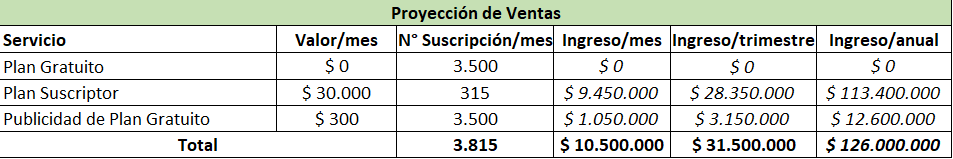
\includegraphics[width=14cm]{Imagenes/ProyeccionVentas.png}
	\label{ProyeccionVentas}
\end{table}

La proyección considera el IPC estimado por el equipo técnico del Banco de la República, con el fin de tener en cuenta la posible inflación y las condiciones relacionadas con el posicionamiento en el mercado y las estrategias de marketing. A continuación, en la tabla \ref{IPCFlujo} se presenta la información indexada teniendo en cuenta dicho indicador.

\begin{table}[H]
	\centering
	\caption[{IPC y flujo de efectivo}]{\centering Tabla del IPC y el flujo de efectivo. \textit{Fuente:} Autores.}
	\includegraphics[width=14cm]{Imagenes/IPCFlujo.png}
	\label{IPCFlujo}
\end{table}

